\section{Introduction}\label{sec:introduction}
Trust plays a key role in interpersonal relationships. For example, a supervisor asks a subordinate to accomplish a task based on several factors that indicate the subordinate can be trusted to do so. When consumers make purchases, they do so with trust that the product will perform as promised. Likewise, when using something like an autonomous vehicle, users must trust it appropriately in order to use it properly. With the rapid advancement of intelligent technology to do tasks that were previously assumed to be too complicated for machines, there is now much discussion in public \cite{Spectrum2016-jv,DeSteno2014-cq,Wagner2016-ck}, business \cite{Banavar2016-nm, Khosravi2016-ke,Tankard2016-rk}, and academic settings \cite{Foley2017-qj,Castelvecchi2016-mr,Lahijanian2016-nd} on how humans can trust said technology -- although, the connection to trust is not always made explicit from a technical standpoint. 

Those who discuss \emph{how} to trust a specific technology are really referring to the need for some indication of the appropriate level of trust to give said technology. In other words, it is desirable to \emph{design} capabilities and methods into intelligent technology which help us achieve appropriate levels of trust in that technology. We refer to these capabilities and methods as as \textit{assurances}. The field of Validation and Verification (V\&V) also uses the term assurances to refer to structured evidence that indicates whether or not a system is functioning according to the design specifications \cite{Calinescu2017-fh}. We'll refer to these assurances as `hard assurances'. Hard assurances are often not relatable to users of systems or used as means for adjusting levels of trust with a user in real-time, but are used for certification and meeting certain qualifications such as safety. This is in contrast to `soft assurances' that are designed that are meant to be used in interaction with users in order to affect their trust and their trust-related behavior. In this paper, `assurances' will refer to soft assurances only.
    
This survey investigates what assurances an Artificially Intelligent Agent (AIA) can provide to a human user in order to affect their trust. The colloquial definitions of `appropriate use', `assurance', `AIA', and `trust' should suffice for now to give the reader a general idea of the motivation; more formal definitions will be presented in Section \ref{sec:background}. There are many researchers, from different disciplines, who will potentially be interested in this work. This includes fields like machine learning, artificial intelligence, robotics and unmanned systems. More broadly, it includes any disciplines that deal in some way with the interface between humans and technology; particularly those who are interested in working with, trusting, interpreting, understanding, and/or regulating AIAs. As such, this paper cuts across multiple disciplines and ties together concepts from several important research topics, such as trustworthy and explainable learning and AI, ethical and transparent autonomy, and safety-/user-aware intelligent systems.

Figure~\ref{fig:SimpleTrust_one_way} is a simple diagram of the trust cycle that exists between a human user and an AIA (justification for this cycle will be presented later): user trust is affected by assurances from the AIA, which in turn affects the user's interaction with the AIA (e.g. to trust AIA with responsibilities, or not). To fully understand and appreciate the importance of assurances, one must have a more formal understanding of its components. This paper provides an overview of the trust cycle components, and then turns more focused attention to assurances, surveying related research to date. From this survey, properties and classifications of assurances are defined, and considerations for further research are presented.

\begin{figure}
    \centering
    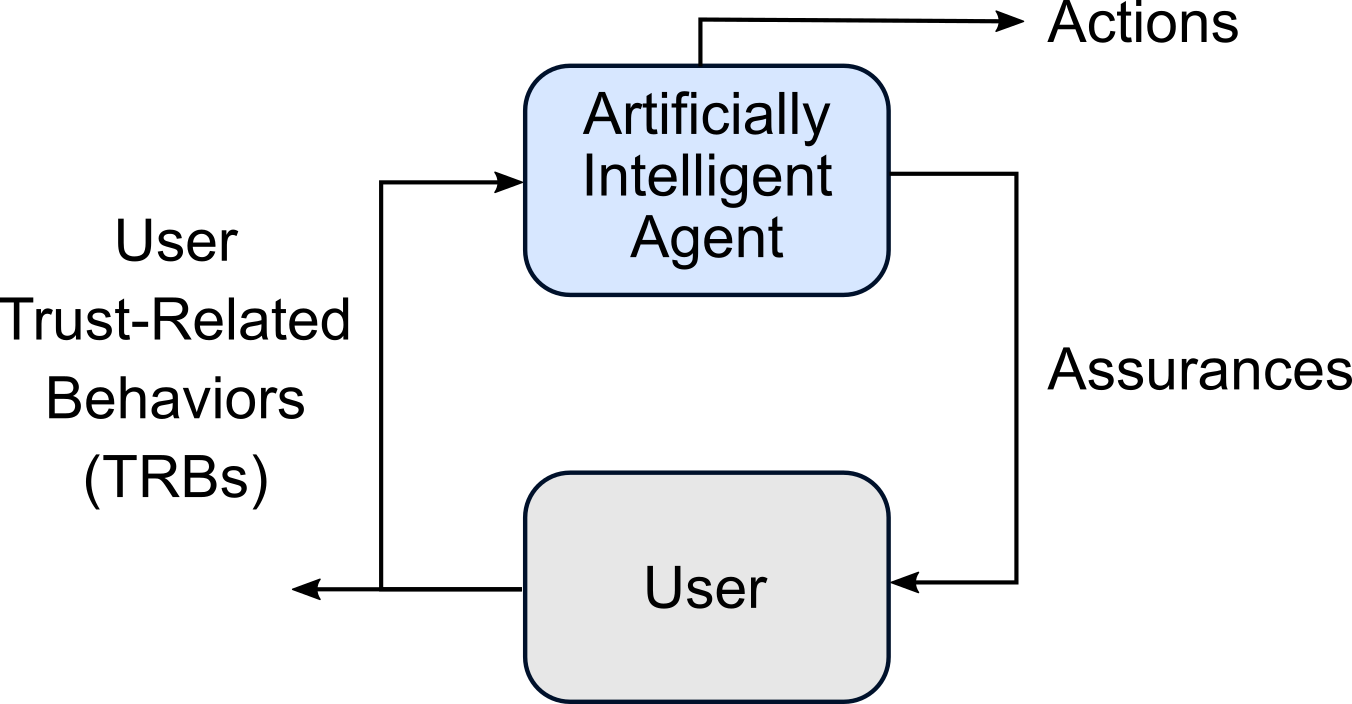
\includegraphics[width=0.5\textwidth]{Figures/SimpleTrust_one_way}
    \caption{Diagram depicting the simple one-way trust development relationship between a human user and an AIA. Based on a user's level of trust they take certain actions (e.g. give AIA commands), these commands can lead the AIA to certain actions and/or to provide assurances to the user in order to affect their trust. Note that some `Task Oriented Behaviors' can fall within the trust cycle, but the addition of a separate arrow is meant to encompass any actions are not trust related.}
    \label{fig:SimpleTrust_one_way}
\end{figure}

Some of the novel contributions of this paper include: identifying several different bodies of research that contribute to this topic; creating a detailed description and definition of assurances in general human-AIA relationships; and making a detailed breakdown of the different components of assurances, and design considerations for implementing them. To this end, Section~\ref{sec:background} provides definitions for each of the terms. In Section~\ref{sec:methodology} we discuss the methodology used when compiling this survey. Section \ref{sec:synthesis} presents a more detailed version of Figure~\ref{fig:SimpleTrust_one_way}, which is derived via surveying related literature. These details highlight methods that have been, and currently are being used to design assurances. Furthermore, via this survey we are able to formally define and classify assurances, which is something that until now has not been done. Finally, recommendations for future work and discussed in Section~\ref{sec:future_work}, and conclusions are presented in Section~\ref{sec:conclusions}.
